%%%%%%%%%%%%%%%%%%%%%%%%%%%%%%%%%%%%%%%%%%%%%%%%%%%%%%%%
%%%%                                              %%%%%%
%%%%  Author: Peter Wilson                        %%%%%%
%%%%                                              %%%%%%
%%%%  Background of shells                        %%%%%%
%%%%                                              %%%%%%
%%%%%%%%%%%%%%%%%%%%%%%%%%%%%%%%%%%%%%%%%%%%%%%%%%%%%%%%

\chapter{DSG technology derivation}
\label{app:DSG technology derivation}
\renewcommand{\Thema}{DSG technology derivation}

The DSG element technology aims to mitigate shear locking in 5-parameter based shell formulations via the concept of discrete shear gaps. This term, coined by Bletzinger et al. \cite{Ble00}, refers to the difference in transverse displacements between a pure 3-parameter Kirchhoff formulation and a 5-parameter Reissner-Mindlin formulation. More explicitly, this concept can be illustrated by considering the deformation of a beam (repeated from section \ref{DSGbackground}):

\begin{figure}[H]
	\subfloat[DSG concept]
	{\label{ref_label1}
	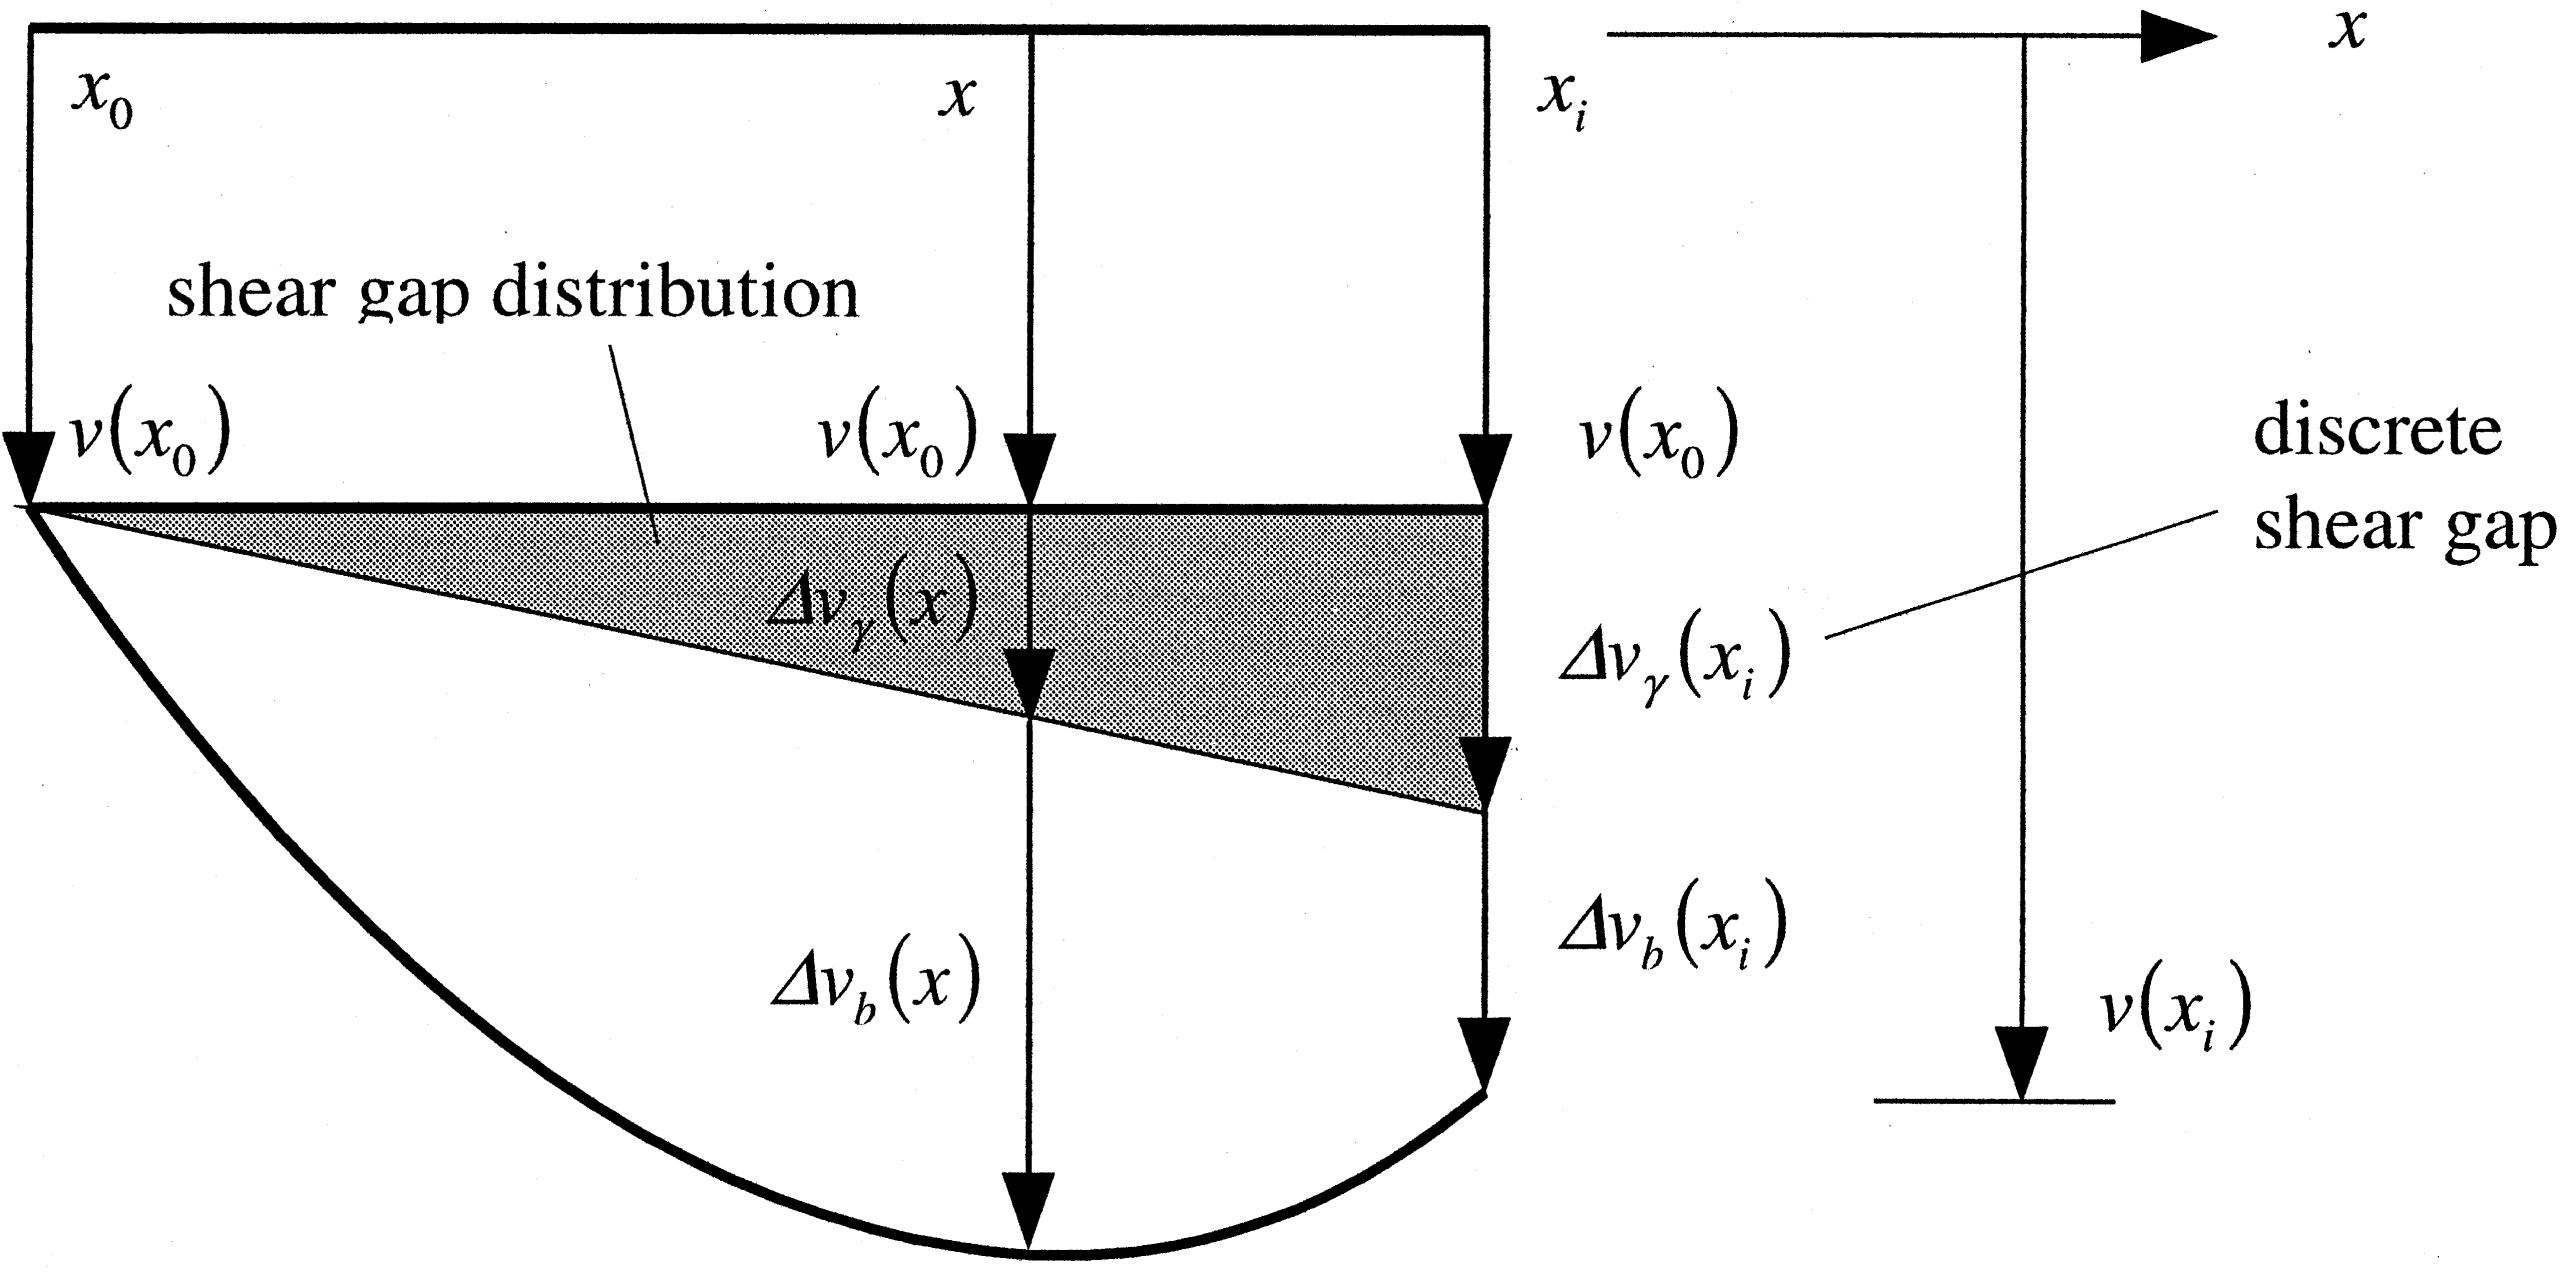
\includegraphics[width=7.3cm]{images/DSG.png}}
	\subfloat[Timoshenko beam kinematics]
	{\label{ref_label1}
		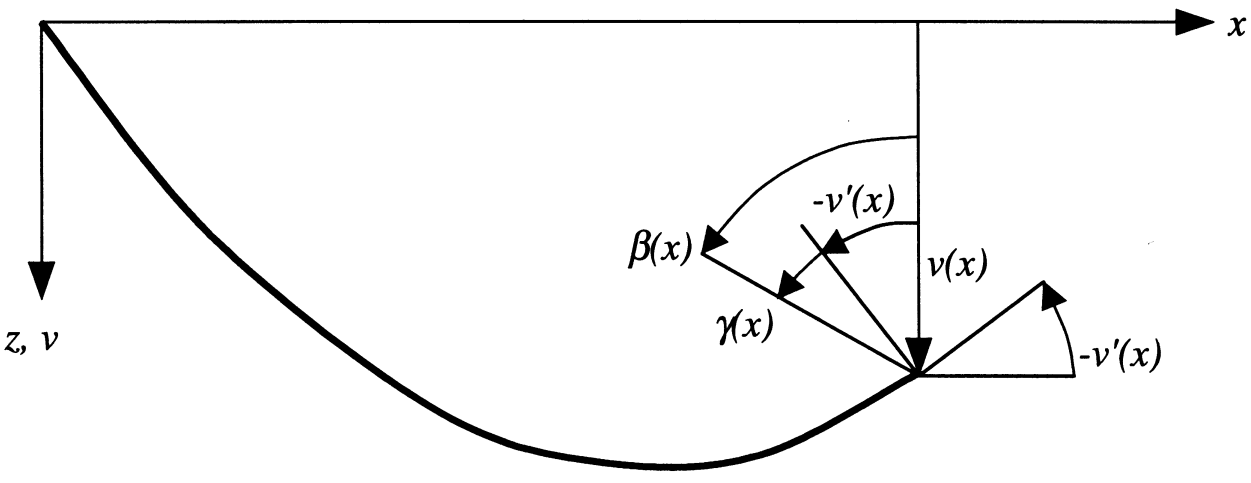
\includegraphics[width=7.3cm]{images/DSG_2.png}}
	\caption{\label{DSG_derivation_pic1}DSG concept and Timoshenko kinematics \cite{Ble00}}
\end{figure}

The shear deformation $\gamma(x)$ of the beam above is defined as the difference between the section rotation $\beta(x)$ and transverse displacement gradient $v'(x)$:
\begin{equation} 
\gamma(x) = v'(x) + \beta(x)
\label{DSG_derivation_0}\ .
\end{equation}

The Bernoulli beam, being the 2D analogue of the Kirchhoff plate, fulfills the condition of vanishing shear deformation:
\begin{equation} 
\gamma(x)_{Bernoulli} = 0 = v'(x) + \beta(x)
\label{DSG_derivation_1}\ .
\end{equation}

The shear deformation field (equation \ref{DSG_derivation_0}) can be discretized into nodal values interpolated with shape functions, typical of the general FEM approach, however, if the same shape functions are used for rotations and transverse displacements, as discussed in section \ref{locking in shell finite elements}, this generally introduces deleterious locking effects. Thus, the novelty of the DSG method, the shear gap, is introduced, which aims to formulate the shear deformation via an integral approach. Considering the 5-parameter formulation analogous Timoshenko beam, the shear gap field $\Delta v_\gamma$ can be recovered by integrating the shear distribution over the element:

\begin{equation} 
\Delta v_\gamma(x) 
= \int_{x_o}^x \gamma \ dx
= v |_{x_o}^x +  \int_{x_o}^x \beta \ dx
\label{DSG_derivation_2}\ .
\end{equation}

Accordingly, the shear gap field can be approximated with shape functions $N_i$ and discrete shear gaps $ \Delta v_{\gamma}^i$ evaluated at each node $i$:

\begin{equation} 
\Delta v_\gamma(x) = \sum_{i=1} N_i \Delta v_{\gamma}^i\ ,
\hspace{10mm} 
\Delta v_\gamma^i 
= \int_{x_o}^{x_i} \gamma \ dx
= v |_{x_o}^{x_i} +  \int_{x_o}^{x_i} \beta \ dx
\label{DSG_derivation_3}\ .
\end{equation}

The shear deformation field may be recovered by differentiating the shear gap field with the onus on the shape functions:

\begin{equation} 
\gamma(x) = \frac{\partial \Delta v_\gamma(x) }{\partial x}
=  \sum_{i=1} \frac{\partial N}{\partial x}\Delta v_{\gamma}^i
\label{DSG_derivation_4}\ .
\end{equation}

With the basic DSG concept established for a simple beam example, the focus can be shifted to the 5-parameter triangular element under development. The general geometry of the element is presented below:

\begin{figure}[H]
	\centering
	\subfloat[3 node triangle with local coordinates]
	{\label{ref_label1}
		\includegraphics[width=6.5cm]{images/DSG_element1.png}}
	\subfloat[3 node triangle with plate theory rotation DOFs]
	{\label{ref_label1}
		\includegraphics[width=7.3cm]{images/DSG_element2.png}}
	\caption{\label{DSG_derivation_pic2}DSG triangle local coordinates and DOFs \cite{Ngu13}}
\end{figure}

At this point it is important to note the current rotation DOF definitions are consistent with plate theory and therefore don't match global Cartesian rotations that follow the right hand rule. The plate theory DOF definitions express shear deformation similar to equation \ref{DSG_derivation_0}:

\begin{equation} 
\begin{pmatrix}
\gamma_x \\
\gamma_y
\end{pmatrix}
=
\begin{pmatrix}
\frac{\partial w}{\partial x} +  \beta_x \\
\frac{\partial w}{\partial y} +  \beta_y
\end{pmatrix}
\label{DSG_derivation_5}\ .
\end{equation}

According to the general form of equation \ref{DSG_derivation_3}, the shear gaps of the triangular element can be determined in parametric space to be:

\begin{equation} 
\Delta v_{\gamma1}^i 
= w |_{\xi_1}^{\xi_i} +  \int_{\xi_1}^{\xi_i} \beta_x a +  \beta_y b \ d\xi
\label{DSG_derivation_6}
\end{equation}
and
\begin{equation} 
\Delta v_{\gamma2}^i 
= w |_{\eta_1}^{\eta_i} +  \int_{\eta_1}^{\eta_i} \beta_x d +  \beta_y c \ d\eta
\label{DSG_derivation_7}\ .
\end{equation}

The rotation fields $\beta_x$ and $\beta_y$ are approximated with nodal values interpolated by the standard linear triangle shape functions:

\begin{equation} 
\beta_\alpha (\xi,\eta)
= \sum_i^3 N_i (\xi,\eta) \beta_\alpha^i
\ ,
\hspace{5mm}
N_1 = 1-\xi-\eta\ ,
\hspace{5mm}
N_2 = \xi\ ,
\hspace{5mm}
N_3 = \eta
\label{DSG_derivation_8}\ .
\end{equation}

Evaluation of the discrete shear gaps at each node yields the following results:

\begin{equation} 
\Delta v_{\gamma1}^1 = 
\Delta v_{\gamma1}^3 = 
\Delta v_{\gamma2}^1 = 
\Delta v_{\gamma2}^2 = 0
\label{DSG_derivation_9}\ ,
\end{equation}
\begin{equation} 
\Delta v_{\gamma1}^2 = 
w_2 - w_1 + \frac{a(\beta_x^1 + \beta_x^2)}{2} + \frac{b(\beta_y^1 + \beta_y^2)}{2}
\label{DSG_derivation_10}
\end{equation}
and
\begin{equation} 
\Delta v_{\gamma2}^3 = 
w_3 - w_1 + \frac{d(\beta_x^1 + \beta_x^3)}{2} + \frac{c(\beta_y^1 + \beta_y^3)}{2}
\label{DSG_derivation_11}\ .
\end{equation}

The shear gap field can be constructed with the discrete nodal shear gaps interpolating shape functions (as per equation \ref{DSG_derivation_8}):

\begin{equation} 
\Delta v_{\gamma \alpha} (\xi,\eta) 
= \sum_i^3 N_i (\xi,\eta) \Delta v_{\gamma \alpha}^i
\label{DSG_derivation_12}\ .
\end{equation}

Finally, shear deformations are determined by differentiating the shear gap field along Cartesian space:

\begin{equation} 
\begin{pmatrix}
\gamma_x \\
\gamma_y 
\end{pmatrix}
=
\begin{pmatrix}
\frac{\partial \Delta v_{\gamma 1}}{\partial \xi}
\frac{\partial \xi}{\partial x}
+
\frac{\partial \Delta v_{\gamma 2}}{\partial \eta}
\frac{\partial \eta}{\partial x} \\
\frac{\partial \Delta v_{\gamma 1}}{\partial \xi}
\frac{\partial \xi}{\partial y}
+
\frac{\partial \Delta v_{\gamma 2}}{\partial \eta}
\frac{\partial \eta}{\partial y}
\end{pmatrix}
\label{DSG_derivation_13}\ ,
\end{equation}

with the inverse Jacobian entries employed above given by:

\begin{equation} 
\mathbf{J}^{-1} = 
\begin{pmatrix}
\frac{\partial \xi}{\partial x} & \frac{\partial \eta}{\partial x} \\
\frac{\partial \xi}{\partial y} & \frac{\partial \eta}{\partial y} \\
\end{pmatrix}
=
\frac{1}{detJ}
\begin{pmatrix}
c & -b \\
-d & a
\end{pmatrix}
\label{DSG_derivation_14}\ .
\end{equation}

The combination of the above equations leads to Bletzinger's \cite{Ble00} linear triangle DSG B matrix:

\begin{equation} 
\begin{pmatrix}
\gamma_x \\
\gamma_y 
\end{pmatrix}
=
\frac{1}{detJ}
\begin{pmatrix}
b-c & \frac{detJ}{2} & 0 & c & \frac{ac}{2} & \frac{bc}{2} & -b & \frac{-bd}{2} & \frac{-bc}{2} \\
d-a & 0 & \frac{detJ}{2} & -d & \frac{-ad}{2} & \frac{-bd}{2} & a & \frac{ad}{2} & \frac{ac}{2}
\end{pmatrix}
\begin{pmatrix}
w_1 \\
\beta_{x1} \\
\beta_{y1} \\
w_2 \\
\beta_{x2} \\
\beta_{y2} \\
w_3 \\
\beta_{x3} \\
\beta_{y3} 
\end{pmatrix}
\label{DSG_derivation_15}\ .
\end{equation}

As noted in figure \ref{DSG_derivation_pic2}, the current B matrix is formulated with respect to rotational DOFs defined as per plate theory, which is not consistent with the Cartesian rotations following the right hand screw rule. To render the DSG formulation in terms of Cartesian rotations suitable for Kratos, the following equivalents can be drawn:
\begin{equation} 
\beta_{yi} = -\theta_{xi}\ ,
\hspace{10mm}
\beta_{xi} = \theta_{yi}
\label{DSG_derivation_16}\ .
\end{equation}

If the preceding equivalents are substituted into equations \ref{DSG_derivation_5} through \ref{DSG_derivation_13} the following B matrix, expressed in terms of Cartesian rotations, is obtained, which matches that of Rama et al. \cite{Ram16}:

\begin{equation} 
\begin{pmatrix}
\gamma_x \\
\gamma_y 
\end{pmatrix}
=
\frac{1}{detJ}
\begin{pmatrix}
b-c & 0 & A & c & \frac{-bc}{2} & \frac{ac}{2} & -b & \frac{bc}{2} & \frac{bd}{2} \\
d-a & -A & 0 & -d & \frac{bd}{2} & \frac{-ad}{2} & a & \frac{-ac}{2} & \frac{ad}{2}
\end{pmatrix}
\begin{pmatrix}
w_1 \\
\theta_{x1} \\
\theta_{y1} \\
w_2 \\
\theta_{x2} \\
\theta_{y2} \\
w_3 \\
\theta_{x3} \\
\theta_{y3} 
\end{pmatrix}
\label{DSG_derivation_17}\ .
\end{equation}
